% Waste is a problem
% Decisionmakers are contemplating many fuel cycle options
% Decisionmakers are contemplating many repository options
% Interfacing between FCO/SA campaign and UFD campaign

\begin{frame}[ctb!]
  \frametitle{Future Disposal System Options}
   \begin{minipage}{0.44\textwidth}
     \begin{figure}[h!]
         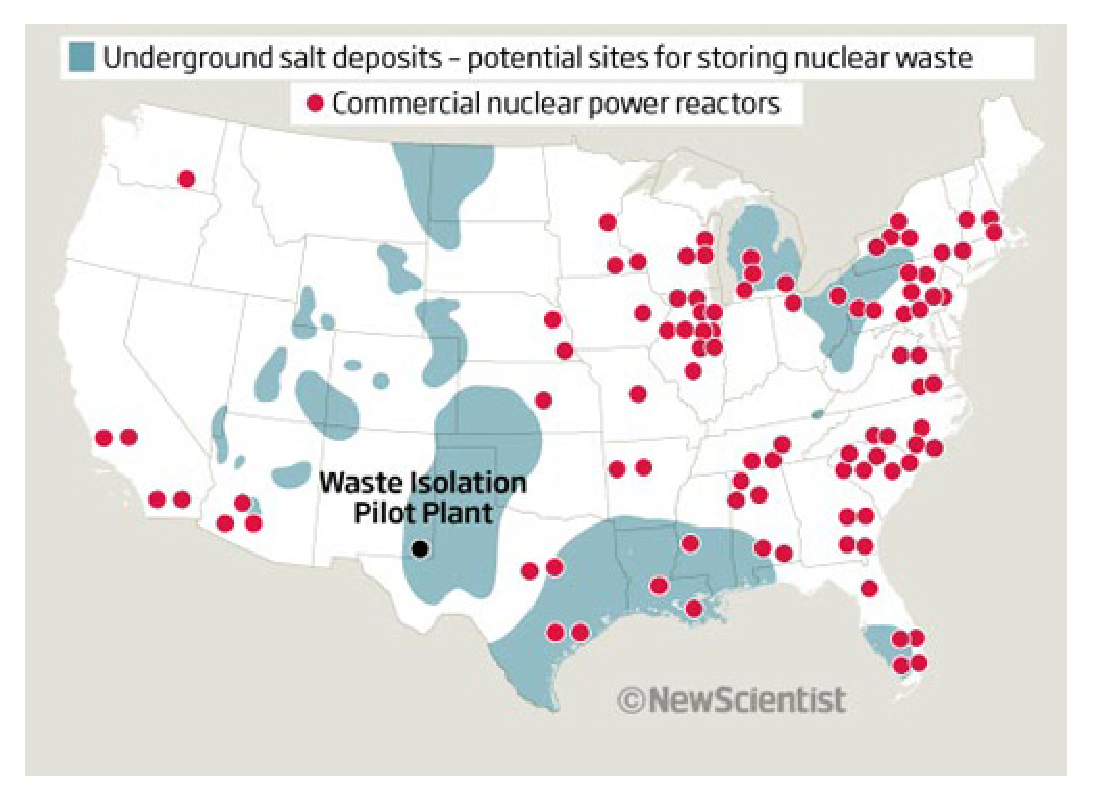
\includegraphics[width=0.8\textwidth]{saltNewScientist.eps}
         \caption{ref. \cite{newscientist_where_2011}}
     \end{figure}
     \begin{figure}[h!]
         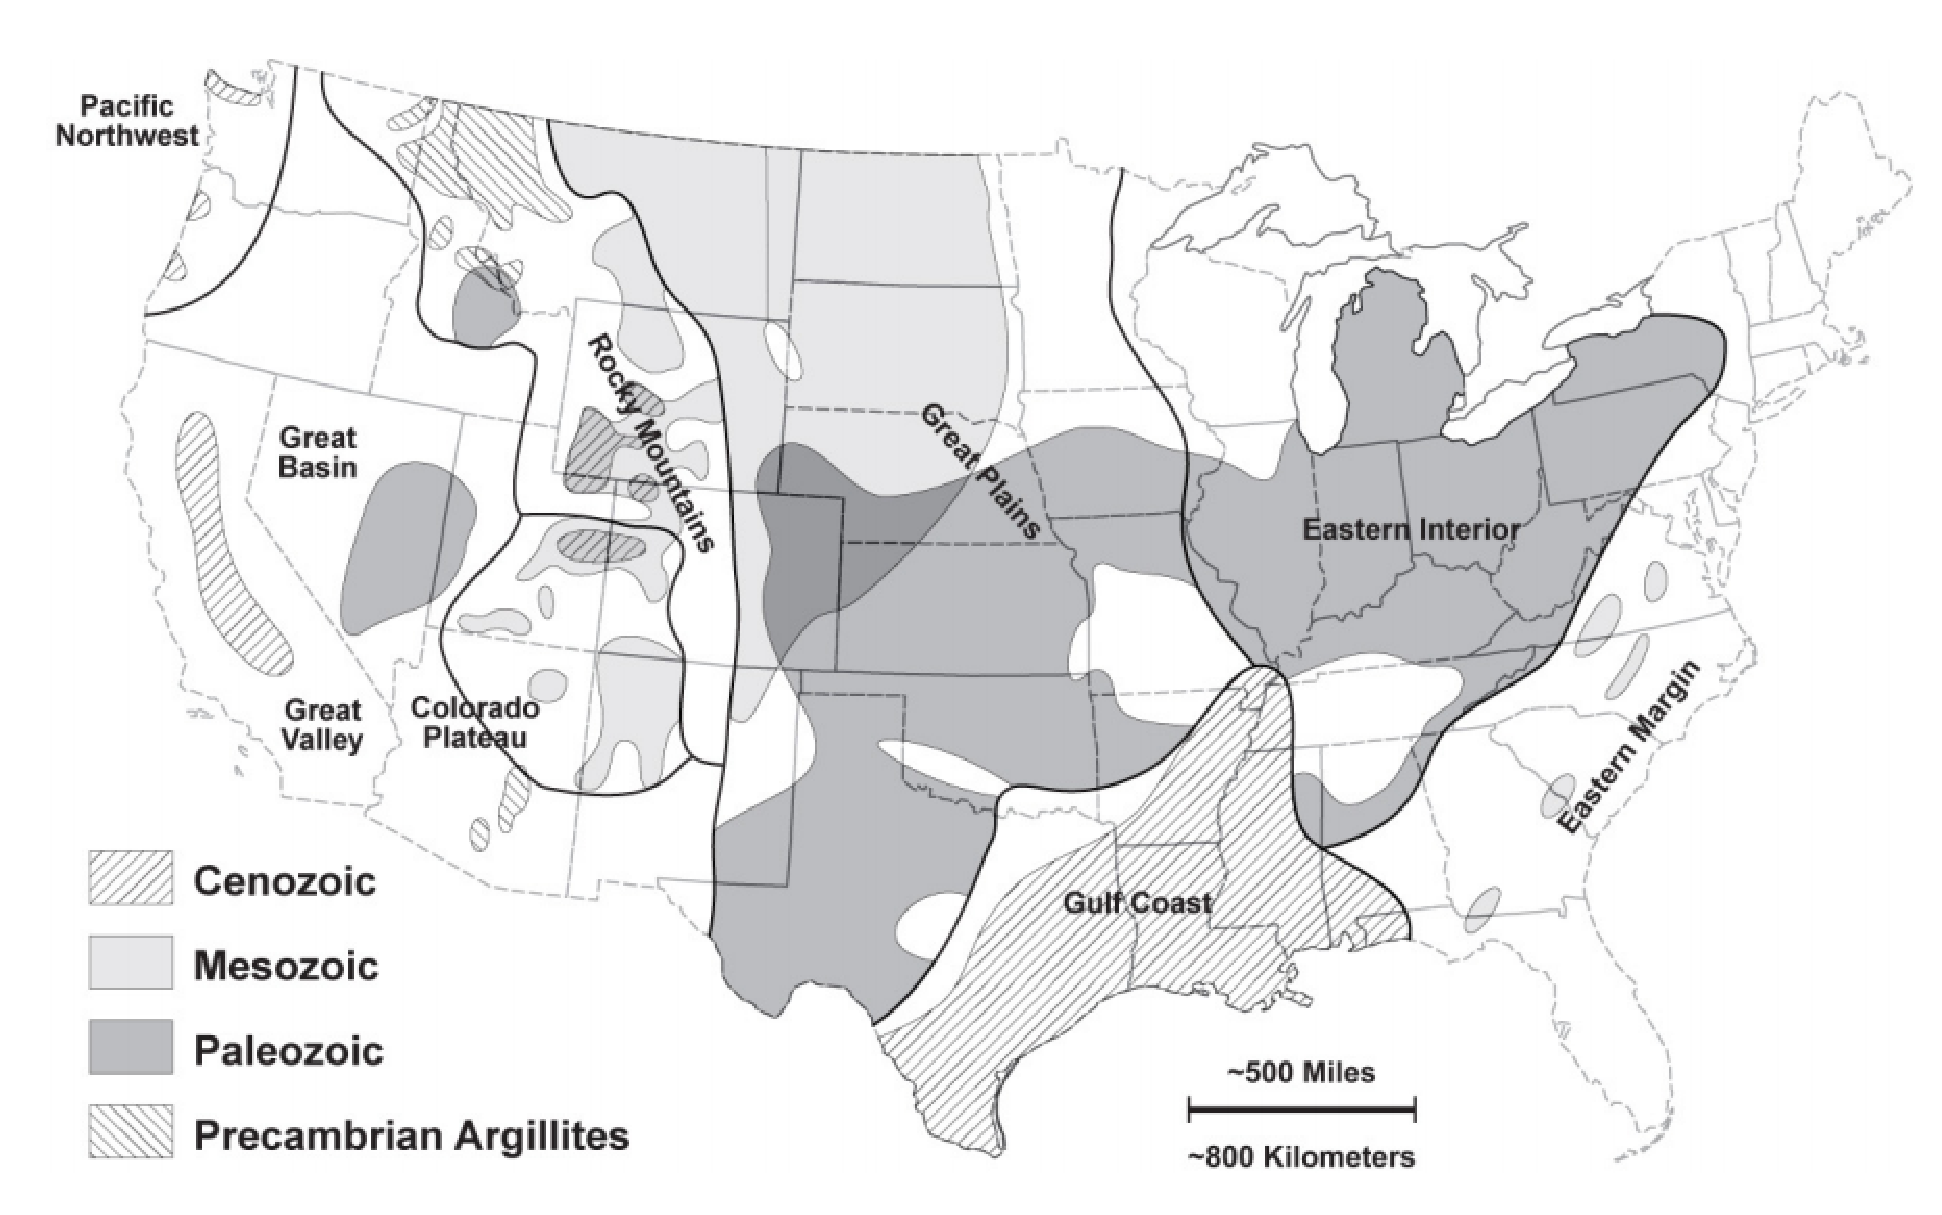
\includegraphics[width=0.8\textwidth]{clayGonzales.eps}
         \caption{ref. \cite{gonzales_shales_1985}}
     \end{figure}
   \end{minipage}
   \hspace{0.01cm}
   \begin{minipage}{0.44\textwidth}
     \begin{figure}[h!]
         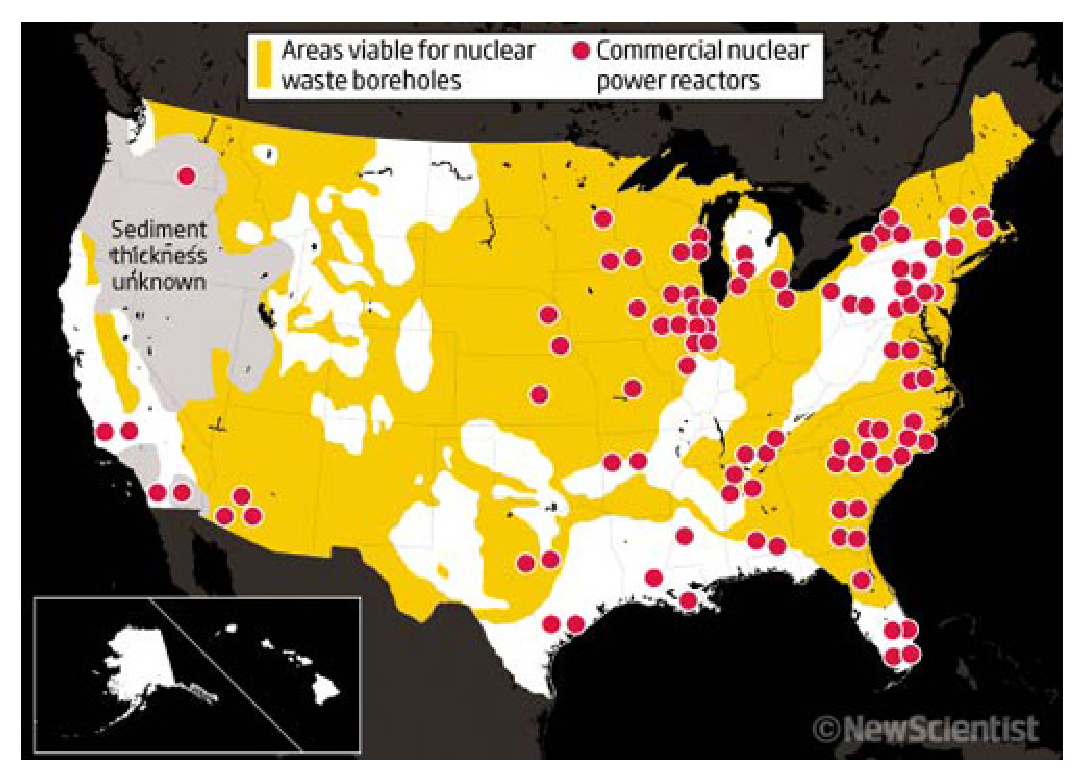
\includegraphics[width=0.8\textwidth]{boreholeNewScientist.eps}
         \caption{ref.  \cite{newscientist_where_2011}}
     \end{figure}
     \begin{figure}[h!]
         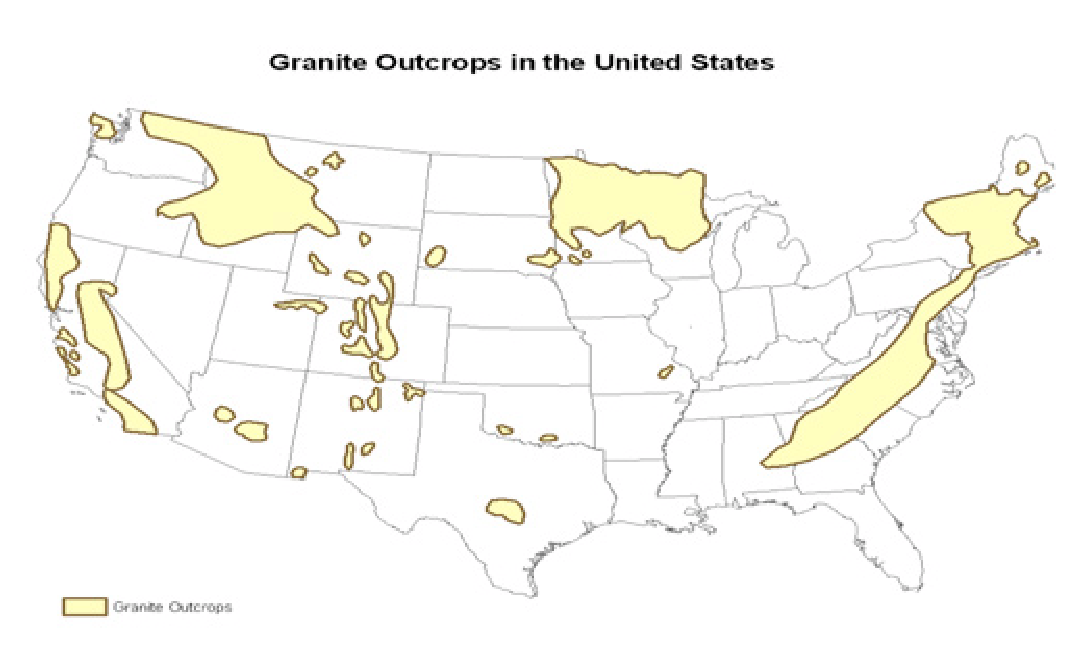
\includegraphics[width=0.8\textwidth]{graniteBush.eps}
         \caption{ref. \cite{bush_economic_1976}}
     \end{figure}
   \end{minipage}
\end{frame}


\begin{frame}[ctb!]
  \frametitle{Future Fuel Cycle Options}
   % Future Fuel Cycles
    \begin{table}
      \centering
      \footnotesize{
      \begin{tabular}{|l|l|l|}
        \multicolumn{3}{c}{\textbf{Domestic Fuel Cycle Options}}\\
        \hline
        Title & Description& Challenges \\
        \hline
        Open          & Once Through      & High Temperatures, Volumes \\
        Modified Open & Partial Recycling & Both high volumes and myriad fuel streams \\
        Closed        & Full Recycling    & Myriad fuel streams \\
        \hline
      \end{tabular}
      \caption[Fuel Cycle Options]{Domestic Fuel Cycle Options }
      \label{tab:fco}
      }
    \end{table}
\end{frame}


